\section*{Overview}

This section introduces the background for the EEW system in place in Japan, consisting of EEW Forecasts and EEW Warnings, and together with the tsunami warnings. Concepts such as intensities, magnitude and epicentres are defined. Two key users and targets are identified, specifically passionate geologists and earthquake-sensitive industries, each having different requirements. A client in the former was interviewed, together with a thorough analysis and comparison of some existing solutions such as SREV, JQuake, KEVI and Quarog. A detailed requirement specification and the critical path is also outlined, consisting of DM-D.S.S. parsing, real-time monitoring, past-earthquake viewing and joint functionalities.

\section{Background Information}

\subsection{The Early Earthquake Warning System}

Earthquake is one of the most common natural disasters in the whole world, and direct consequences of earthquakes include tsunamis which could be catastrophic.

Japan, sitting on the intersection of the Eurasian, the Philippine and the North-American plates, is the countries with most earthquakes. Historically, the Great Kant\=o Earthquake (関東大震災) in 1923, the Great East Japan Earthquake (東日本大震災) in 2011 (a.k.a. the T\=ohoku Earthquake) and the recent 2024 Noto Peninsula Earthquake (能登半島地震) all caused hundreds of deaths, both due to the result of the earthquake(s) and the resulting tsunami.

To provide protection to its residents, the \href{https://www.jma.go.jp/jma/index.html}{Japan Meteorological Agency} (JMA, 気象庁), together with the \href{https://www.bosai.go.jp}{National Research Institute for Earth Science and Disaster Resilience (NIED, 防災科研)} placed thousands of \textbf{earthquake sensors} across Japan (the Hi-net, the K-NET, the KiK-net and the F-NET), with several of them lying deep in the sea bed, measuring displacement, velocity and acceleration, which are connected to multiple servers, including two located in \=Osaka and T\=okyo.

Using data obtained from the sensors, computers do some complicated algorithms (mentioned below) to send out \textbf{early earthquake warnings (EEWs, 緊急地震速報)} automatically within milliseconds. There are two types of EEWs:
\begin{enumerate}
    \item \textbf{EEW (Forecast, 予報).} Sent out to \textbf{highly-dependent industries} (e.g. rail industry, power plants) and \textbf{subscribed users}, when maximum intensity level of more than 3, or a magnitude of more than 3.5 is expected.
    \item \textbf{EEW (Warning, 警報).} Sent out to \textbf{everyone} via TV, Radio, Mobile Phone, SMS, etc., when a maximum intensity level of more than 4 is expected.
\end{enumerate}

After the earthquake, JMA staff will determine the location and severity of tsunami warnings to be issued, if necessary.

\subsection{Earthquake Terminology}

\begin{itemize}
    \item \textbf{Intensity (震度).} The intensity describes the intensity vibration of a point due to an earthquake. It is not unique to an earthquake - \textbf{different places can have different intensities} due to the distance to the epicentre, and intensity will also change over time. JMA measures intensity using \textbf{9 levels: 1, 2, 3, 4, 5--, 5+, 6--, 6+ and 7} in increasing order.
    \item \textbf{Magnitude/Scale.} The magnitude of an earthquake describes the energy released in the earthquake in a logarithmic scale. \textbf{It is unique to an earthquake.}
    \item \textbf{Epicentre/Hypocentre.} The epicentre is the surface point directly above the true centre of the earthquake.
    \item \textbf{Focal Depth.} The focal depth is the depth of the true centre of the earthquake.
    \item \textbf{P-Wave and S-Wave.} These are seismic waves, sourced from the true centre of the earthquake, travelling at different speeds, with Primary (P)-Wave travelling faster and Secondary (S)-Wave travelling slower.
\end{itemize}

\section{Problem Area}
The main goal of this application is to provide a visualisation of the earthquake/tsunami related data feed(s) provided by JMA's affiliated institution, \href{https://dmdata.jp}{Disaster Mitigation Data Send Service (DM-D.S.S)}. There are numerous apps providing a list of recent earthquakes, the real-time data measured by the sensors, and the real time earthquake warning displayed on a map, but rarely are there good apps that combine all those features together satisfyingly, with just the necessary features the author needs.

Some applications are no longer being updated due to change in the user's policy of the related data feed. Furthermore, most of the apps available are only in Japanese, not in English or my home language Chinese, which can create trouble for the author to understand.

\section{Client and End User}
The primary target of this application will be passionate geographers and geologists who are interested in the study of earthquake observations and predictions. The age group of this vary all the way from primary-school students to adults, including the author who has been amazed by the technology since the age of 12. They could take any employment, ranging from students to full-time jobs. Their proficiency usually varies, since there are people new to this field who probably does not have much knowledge, so the interface of the application should be relatively user-friendly and understandable, hiding unnecessary technical complexities.

Another target client could be industries which highly rely on earthquake predictions due to the risk imposed by earthquakes. High-speed railway and nuclear power plants are good examples of this. Therefore, the staff in charge monitoring will usually have higher proficiency and would like more detailed data of the earthquake. However, they will only need the necessary data from earthquakes happening close to them and only require intensity data of the point in interest (e.g. the power plant). To put this into content, an earthquake happening 1000 km away from them does not need to be fed into their system, while they would like to see the intensity of the shock and the arrival time of the seismic waves to decide the actions. In fact, the author really likes investigating on the rail industry, whose infrastructure could be greatly affected by earthquakes.

Table \ref{tab:users} compares relative features of these two target users/clients.

\begin{table}[!ht]
    \centering

    \begin{tabular}{|c|l|p{0.36\linewidth}|}
        \hline
        Feature              & Primary Target                     & Secondary Target                                          \\
        \hline\hline
        Description          & Passionate Geologists              & Earthquake-Sensitive Industries                           \\
        Age                  & Varies (Middle School -- Adults)   & Work Age                                                  \\
        Reason               & Monitor Live \& Latest Earthquakes & Monitor Risks to Infrastructure                           \\
        Proficiency          & Varies (Beginner -- Amateur)       & Trained Professional                                      \\
        General Requirements & Monitor Overall Movement           & Alert about intensity and arrival time at specific points \\
        \hline
    \end{tabular}

    \caption{Comparison of target users and clients}
    \label{tab:users}
\end{table}

\section{Research Methodology}
\subsection{Client Interview}
The author interviewed my friend Wesley Ma, who is a passionate geologist on earthquake studies and also monitor earthquakes regularly.

\begin{enumerate}
    \item \textit{Which earthquake monitoring apps do you use?}

          \textbf{Response:} JQuake, SREV, Quarog, KEVI, Kyoshin-Monitor (Support discontinued), Kiwi Monitor (Support discontinued)

    \item \textit{Do you subscribe/pay to services such as DM-D.S.S. to use earthquake monitoring apps, and do you think it is worth the price?}

          \textbf{Response:} Yes. However, DM-D.S.S. is a little expensive. However, the price becomes more affordable considering the information provided by the subscription.

    \item \textit{Do you watch YouTube livestreams on earthquake monitoring?}

          \textbf{Response:} I do not usually watch the live streams, as almost no one who has already has a monitoring app will use the stream. They provide mostly the same information as the applications, just real-time streaming the windows.

    \item \textit{Why do you use earthquake monitoring apps?}

          \textbf{Response:} To monitor the earthquake. This is derived from my interest in broadcasting culture in Japan. This eventually led me to be intrigued with the development of earthquake monitoring technologies and theories in Japan.

    \item \textit{How often do you use earthquake monitoring apps (e.g. all the time/after school/only after big earthquakes)?}

          \textbf{Response:} After big earthquakes. But I usually open one or two apps for all-day monitoring to catch potential major (or medium) earthquakes.

    \item \textit{Describe the advantages and disadvantages of each of them, mentioning the specific features.}

          \textbf{Response:}
          \begin{itemize}
              \item SREV is a good one, but it is only available in a browser with no app.
              \item Kyoshin-Monitor and Kiwi Monitor are relatively more stable, but the source is not the same as that from the former two apps, and its support is also discontinued.
              \item Quarog has weak response time and interacting interface.
              \item JQuake is the most developed app, which includes nearly all functions that can be thought of. However sometimes the connection of WebSocket is unstable.
              \item KEVI does not have the sound files configured by default. Some information are not displayed clearly enough.
          \end{itemize}

    \item \textit{What features do you use the most/least?}

          \textbf{Response:} Basic earthquake notifications, and should be including sufficient and prompt information.

    \item \textit{What features are redundant in the earthquake monitoring apps you use?}

          \textbf{Response:} KEVI has a weather monitoring function, which could be redundant. But that could be caused by the different purposes of the app. Hence, no further comments. It is not a bad thing.

    \item \textit{What are the critical features of an earthquake monitoring app?}

          \textbf{Response:} To provide accurate, prompt and detailed information according to the source released by the JMA, the information display interface should be easy to read and understand. This is not only helping the people who like to monitor, but more importantly, provides the easiest way to the people who really need to seek information to minimise the harm brought by earthquakes and successive disaster.

    \item \textit{What additional features would you like to have in those existing apps?}

          \textbf{Response:} Summarise all the useful features from different apps into one app. Stable connection. Nothing else.
\end{enumerate}

\subsection{Existing Applications and Solutions}

Based on the applications the author uses and the feedback from interviewee, there are the following commonly-used applications:
\begin{itemize}
    \item \href{https://jquake.net}{JQuake}
    \item \href{https://kotoho7.github.io/scratch-realtime-earthquake-viewer-page/}{Scratch Real-time Earthquake Viewer (SREV)}, available in compiled form at \GitHubHref{kotoho7}{scratch-realtime-earthquake-viewer-page}
    \item \href{https://svs.ingen084.net/kyoshineewviewer/}{Kyoshin EEW Viewer for Ingen (KEVI)}, available at \GitHubHref{ingen084}{KyoshinEewViewerIngen}
    \item \href{https://fuku1213.github.io/quarog-site/}{Quarog}
\end{itemize}

\subsubsection{Supported Platforms}

Supported platforms of those apps are listed in Table \ref{tab:exist-platform}. In particular, note that SREV is a web-based and GitHub Pages-hosted application therefore supporting all platforms. KEVI is written in .NET Framework and supports the second most platforms, with JQuake not supporting Linux and Quarog only supporting Windows.

\begin{table}[!ht]
    \centering
    \begin{tabular}{|c||c|c|c|c|}
        \hline
        Platform    & JQuake     & SREV       & KEVI       & Quarog     \\
        \hline
        Windows     & \checkmark & \checkmark & \checkmark & \checkmark \\
        macOS       & \checkmark & \checkmark & \checkmark &            \\
        Linux       & \checkmark & \checkmark & \checkmark &            \\
        Android/iOS &            & \checkmark &            &            \\
        \hline
    \end{tabular}
    \caption{Supported platforms of existing solutions}
    \label{tab:exist-platform}
\end{table}

\subsubsection{Earthquake Monitoring}

An overview feature table of monitoring is included in Table \ref{tab:exist-monitoring}. In particular, note that due to the nature of SREV being Scratch-programmed and web-based, it reached a special agreement with DM-D.S.S. to use the API without the need of all users paying for this, since it is hard to integrate such function into a web application.

Quarog is a relatively new application and only supports basic functionalities of EEW Viewing and past earthquake listing, as shown in Figure \ref{fig:quarog-monitor-features}. JQuake is solely dedicated to earthquake and tsunami monitoring as shown in Figure \ref{fig:jquake-monitor-features}, while KEVI has features like rain clouds map and natural disaster warning which is beyond the scope of this analysis (which is a burden to users only requiring earthquake monitoring and a waste of storage space).

It is worth noting that for SREV, DM-D.S.S. is integrated with special permission with no login required. For JQuake, although it has tsunami warnings/special warnings, the tsunami forecast is not available.

\begin{table}[!ht]
    \centering

    \begin{tabular}{|c||c|c|c|c|}
        \hline
        Feature                        & JQuake     & SREV       & KEVI       & Quarog     \\
        \hline
        NIED Real-time Shake Support   & \checkmark & \checkmark & \checkmark &            \\
        DM-D.S.S. WebSocket Support    & \checkmark & \checkmark & \checkmark & \checkmark \\
        Real-time Sensor Data          & \checkmark & \checkmark & \checkmark &            \\
        Vibration Alert                & \checkmark & \checkmark & \checkmark &            \\
        Past Earthquake List           & \checkmark & \checkmark & \checkmark & \checkmark \\
        Past Earthquake Details        &            & \checkmark & \checkmark & \checkmark \\
        Tsunami Warning                & \checkmark & \checkmark & \checkmark &            \\
        Real-time EEW                  & \checkmark & \checkmark & \checkmark & \checkmark \\
        Calculated Seismic Wavefronts  & \checkmark & \checkmark & \checkmark & \checkmark \\
        User-Defined Key Monitor Point & \checkmark &            & \checkmark &            \\
        Sub-Map for the Okinawa Area   & \checkmark &            & \checkmark &            \\
        Replay                         & \checkmark &            & \checkmark &            \\
        \hline
    \end{tabular}

    \caption[Feature comparison in monitoring of existing solutions]{Feature comparison in monitoring of existing solutions}
    \label{tab:exist-monitoring}
\end{table}

\begin{figure}[!ht]
    \centering

    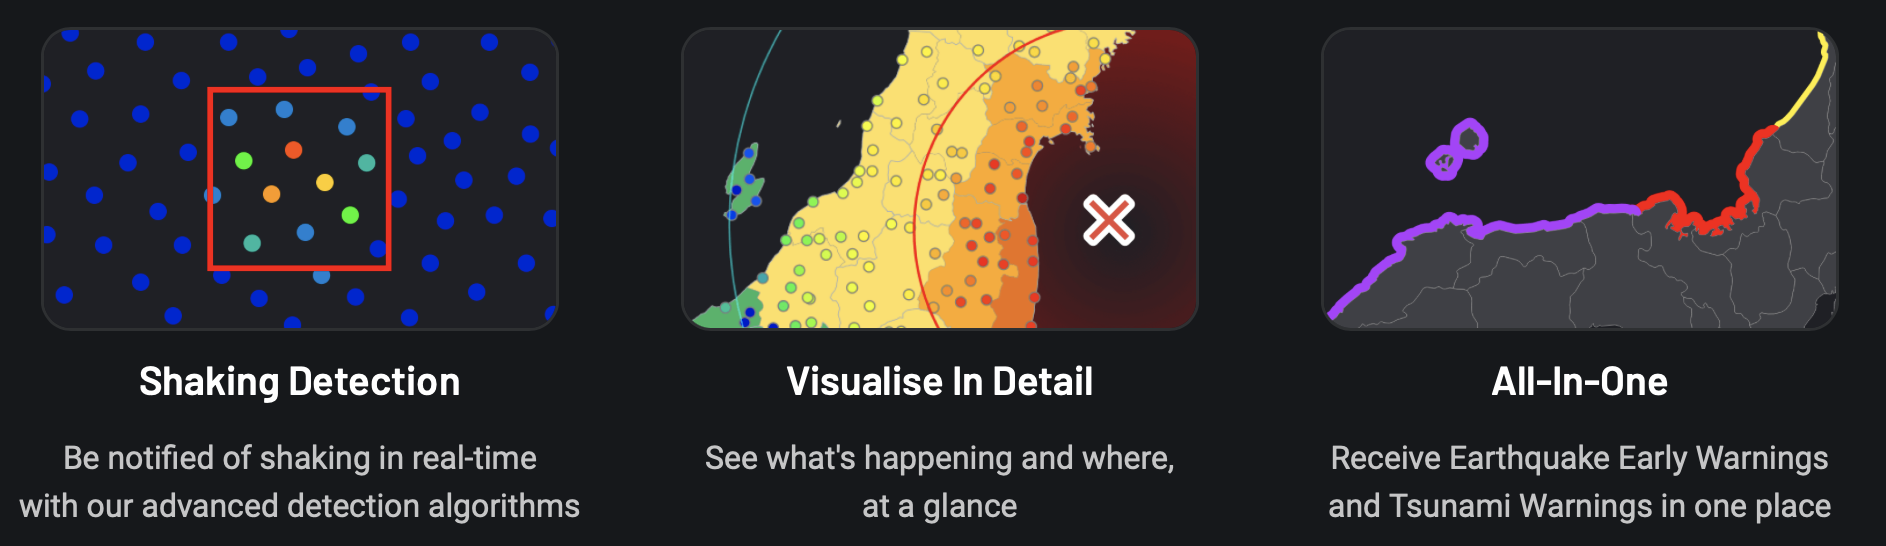
\includegraphics[width=0.6\linewidth]{jquake-features.png}
    \caption[Feature introduction of JQuake]{Feature introduction of JQuake, screenshot from website.}
    \label{fig:jquake-monitor-features}
\end{figure}

\begin{figure}[!ht]
    \centering

    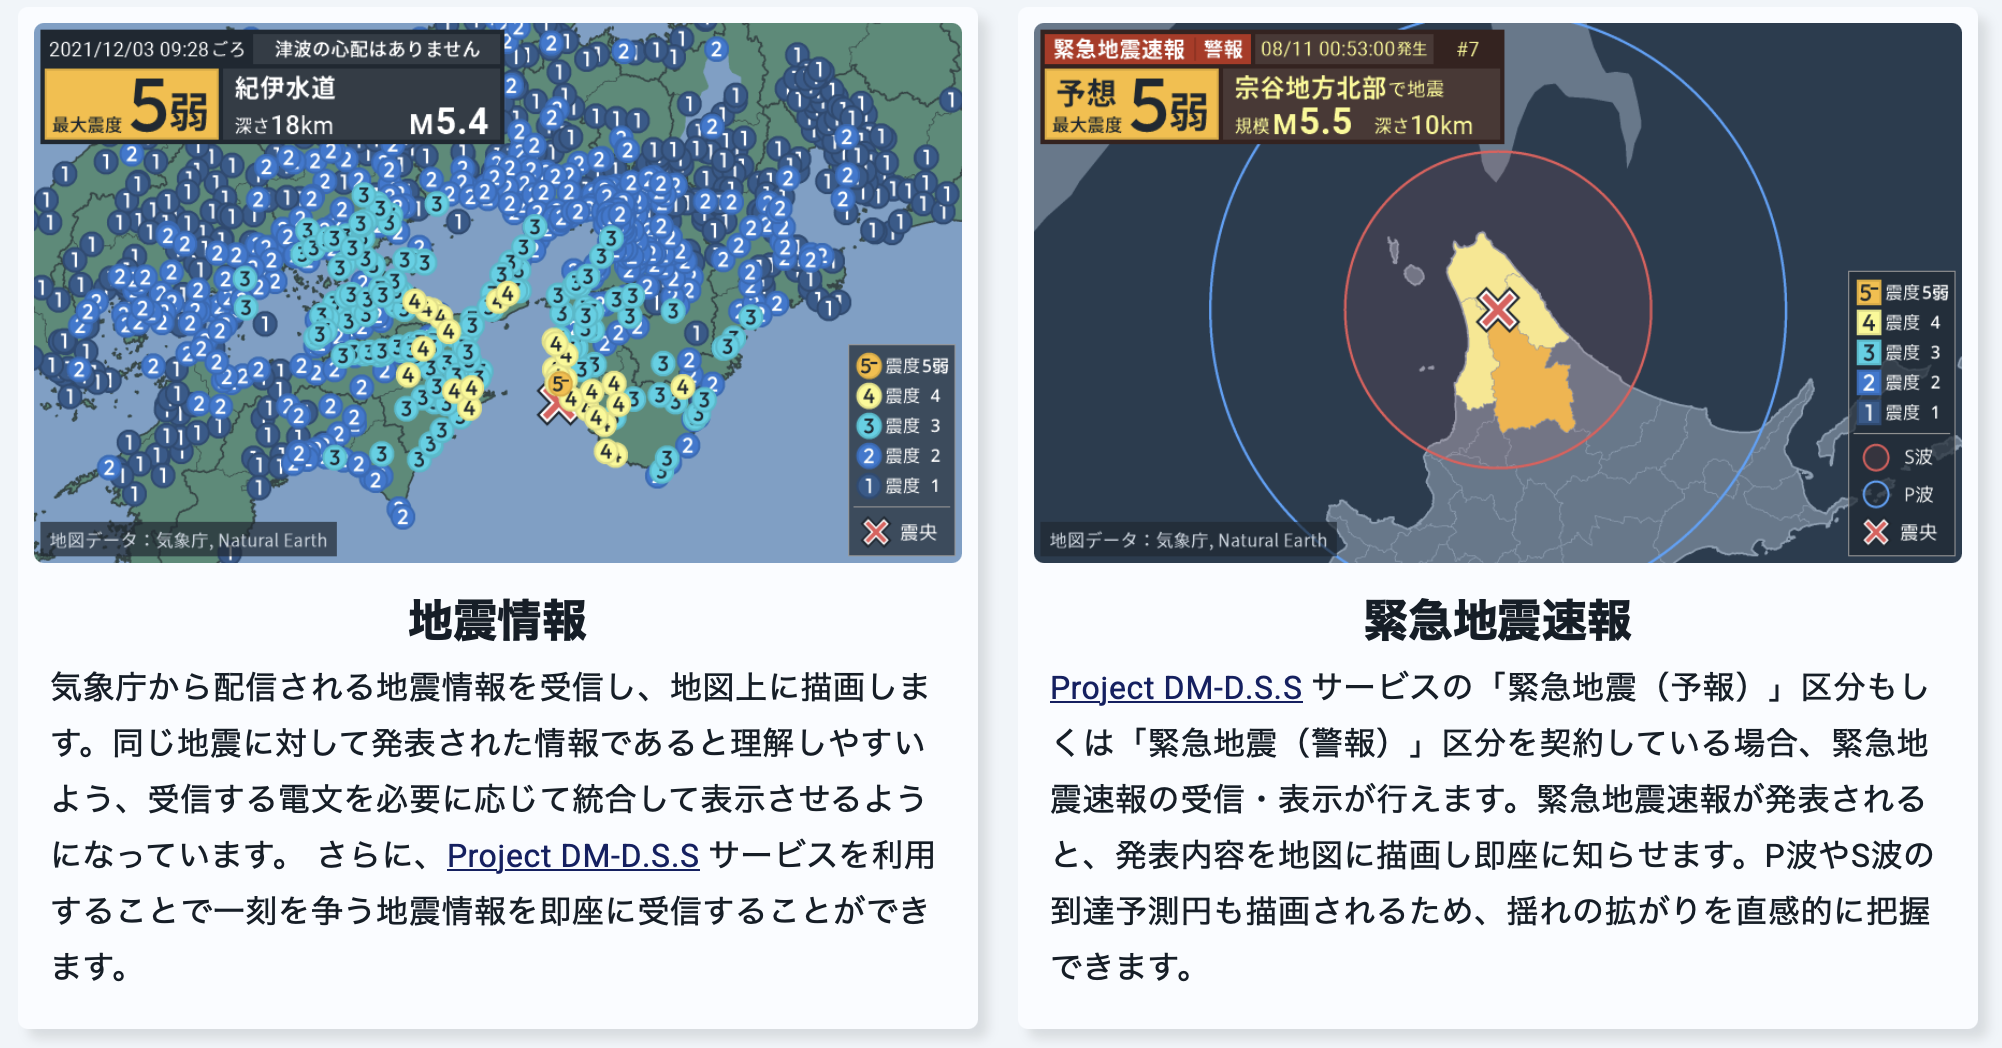
\includegraphics[width=0.6\linewidth]{quarog-features-1.png}\\
    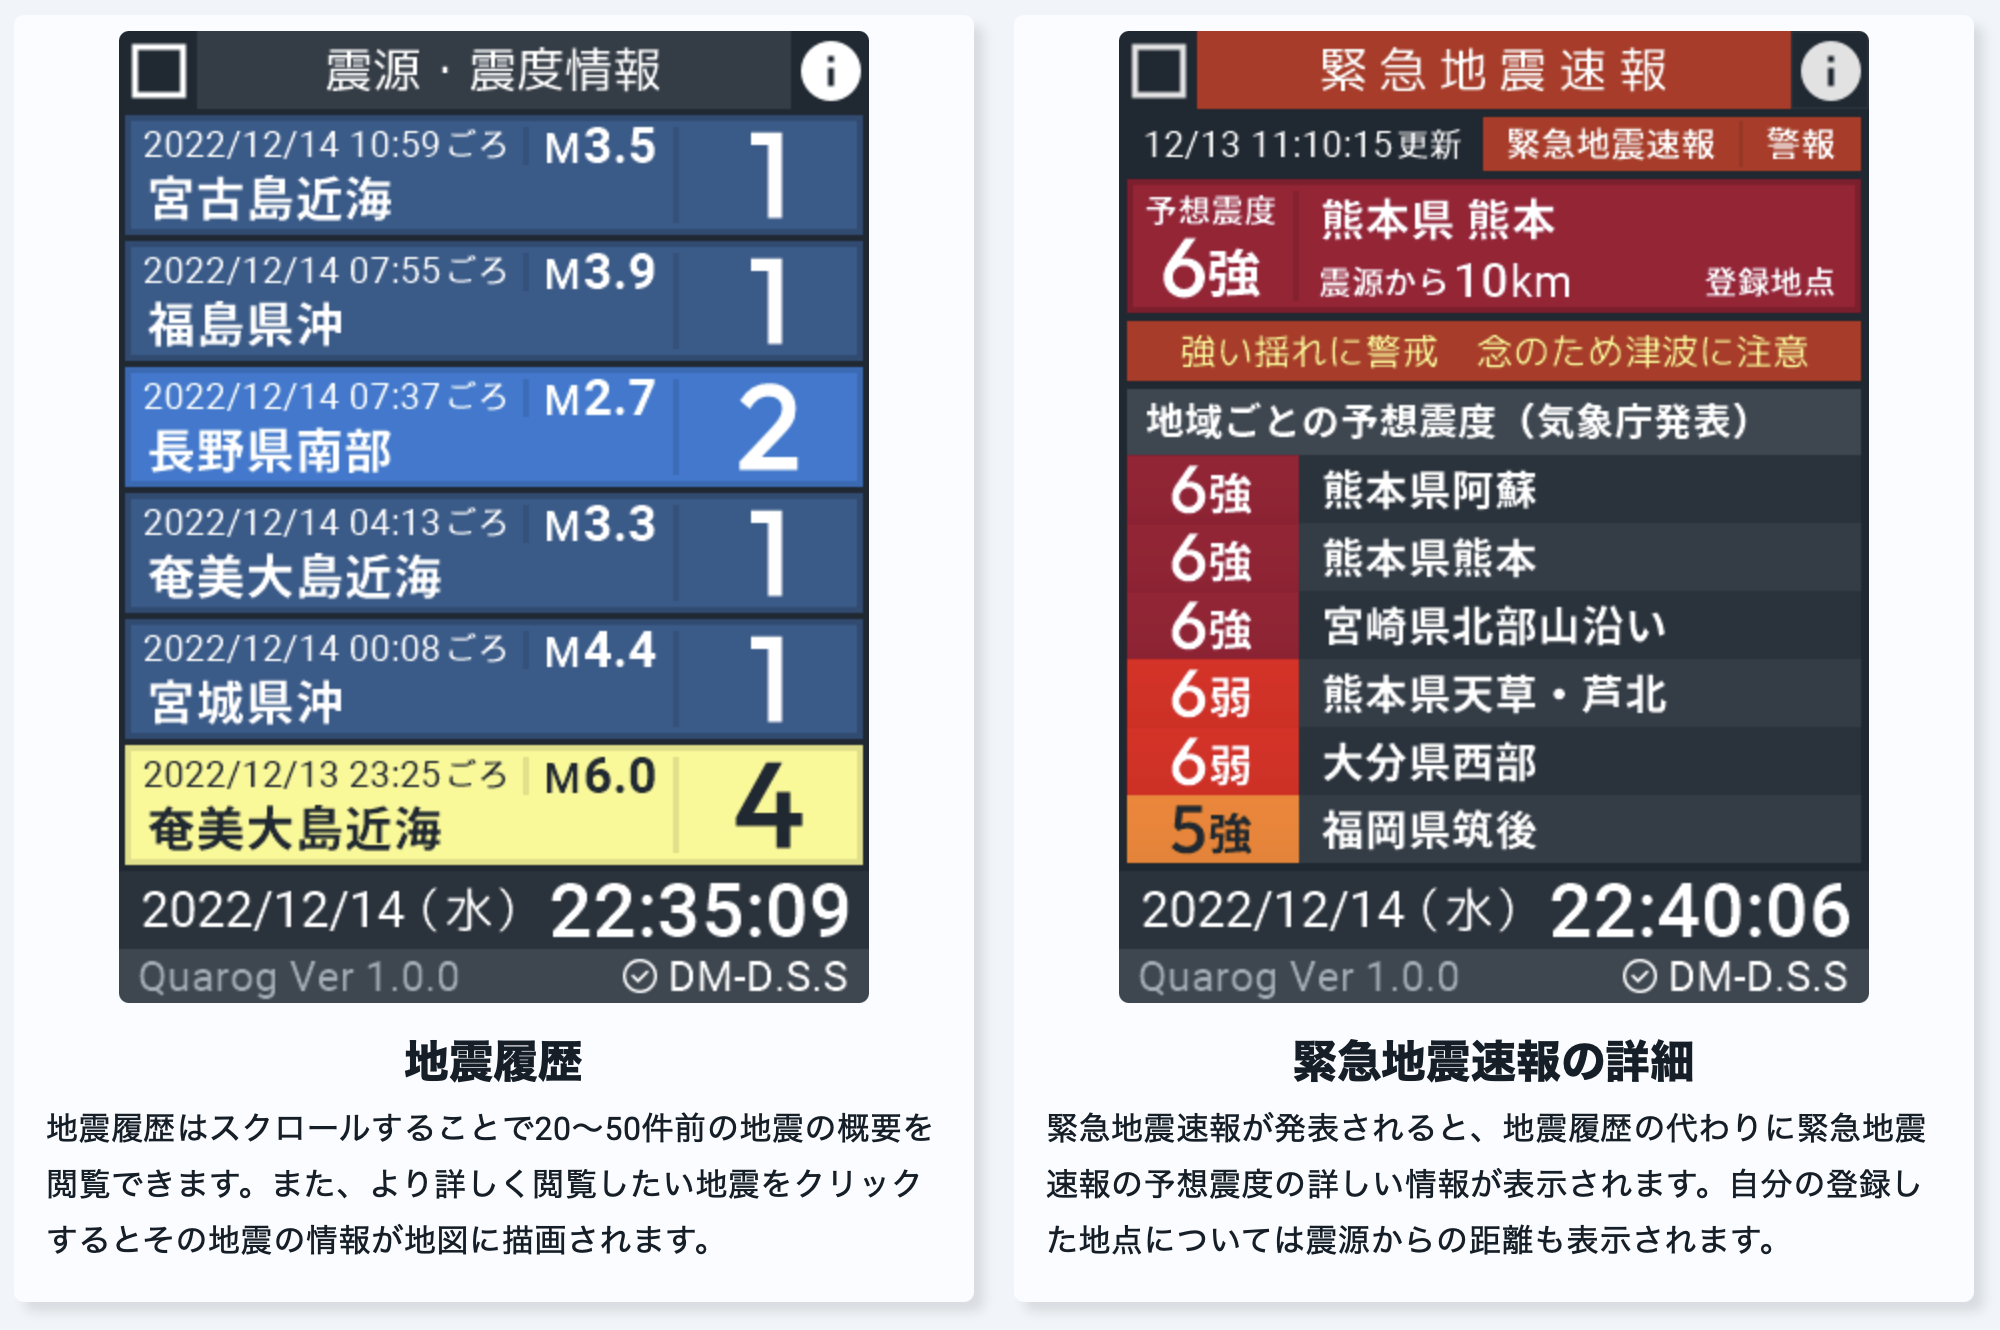
\includegraphics[width=0.6\linewidth]{quarog-features-2.png}
    \caption[Feature introduction of Quarog]{Feature introduction of Quarog, screenshot from website.\\Top-left: Past earthquake information; Top-right: Real-time EEW;\\Bottom-Left: Past earthquake list; Bottom-Right: Details of EEW.}
    \label{fig:quarog-monitor-features}
\end{figure}

\subsubsection{Configuration Options}

There are also a variety of configuration options available for all apps, as listed in Table \ref{tab:exist-config}. Both KEVI and Quarog supports the adjustment of the colour theme, and Quarog even supports changing the style of how blocks are displayed and coloured as shown in Figure \ref{fig:kevi-colour-cust} and \ref{fig:quarog-cust}. Playing a sound on the speaker is also common among the apps to remind the user of earthquakes.

\begin{table}[!ht]
    \centering

    \begin{tabular}{|c||c|c|c|c|}
        \hline
        Feature             & JQuake     & SREV       & KEVI       & Quarog     \\
        \hline
        DM-D.S.S. Login     & \checkmark &            & \checkmark & \checkmark \\
        Sound Alert         & \checkmark & \checkmark & \checkmark & \checkmark \\
        System Notification &            &            & \checkmark &            \\
        Colour Theme        &            &            & \checkmark & \checkmark \\
        Map Colouring Style &            & \checkmark &            & \checkmark \\
        \hline
    \end{tabular}
    \caption{Feature comparison in configuration and customisability of existing solutions}
    \label{tab:exist-config}
\end{table}

\begin{figure}[!ht]
    \centering

    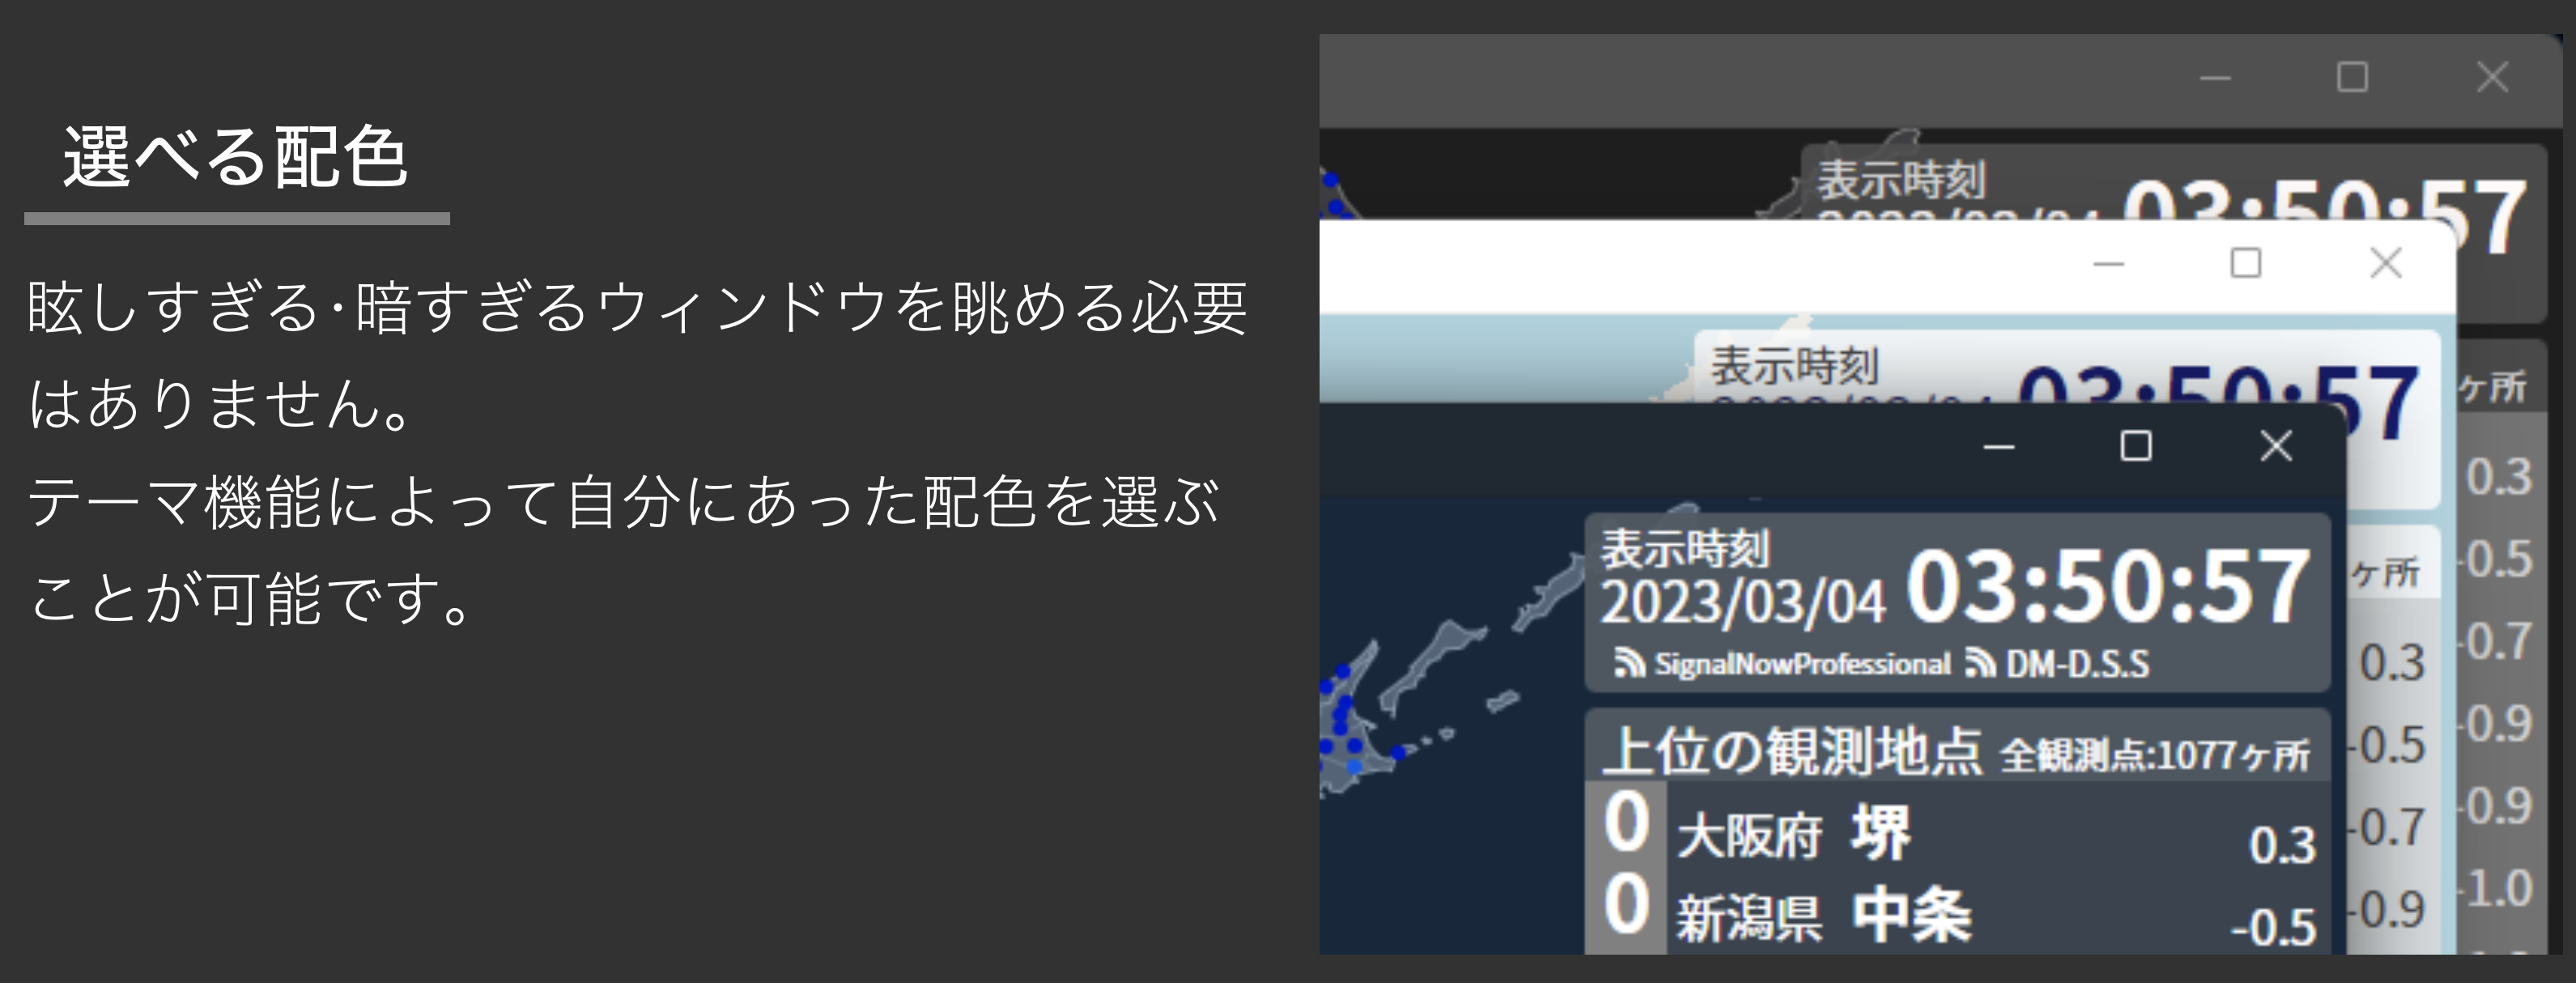
\includegraphics[width=0.5\linewidth]{kevi-colour.png}
    \caption[Customisable colour scheme of KEVI]{Customisable colour scheme of KEVI, screenshot from website.}
    \label{fig:kevi-colour-cust}
\end{figure}

\begin{figure}[!ht]
    \centering

    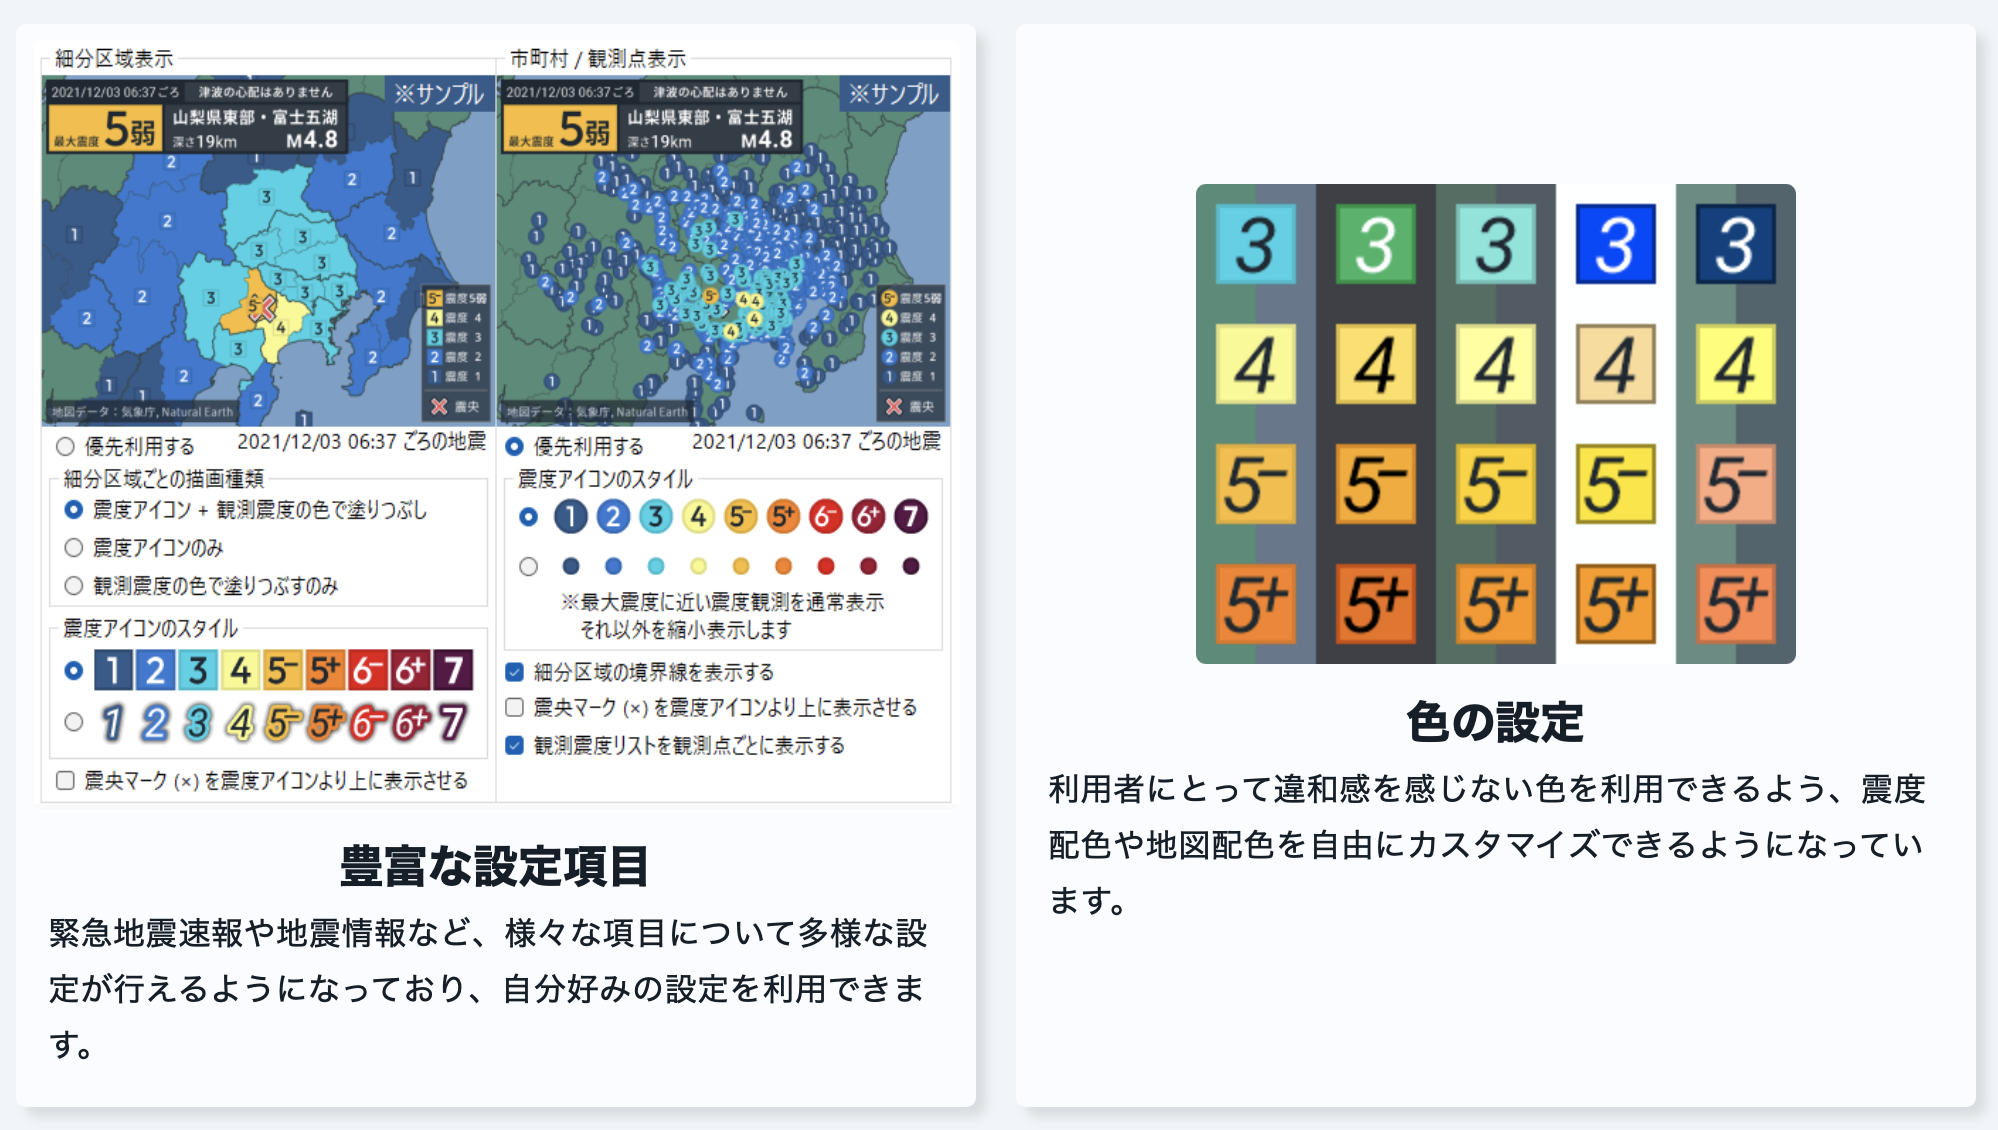
\includegraphics[width=0.6\linewidth]{quarog-cust.png}
    \caption[Customisability of Quarog]{Customisability of Quarog, screenshot from website.}
    \label{fig:quarog-cust}
\end{figure}

% TODO: Include analysis on GUI

\section{Features of proposed solution}

Based on the potential user/client interview results, and the research into the existing solutions, the following key features should appear in the solution, since they are essential to earthquake monitoring applications:
\begin{enumerate}
    \item DM-D.S.S. Login functionality (for the data source)
    \item Real-Time Sensor Shake Intensity Data (w/ vibration alert)
    \item EEW Visualisation (w/ Calculated Seismic Wavefronts)
    \item Past Earthquake List (w/ Option to review details)
    \item Tsunami Warning Visualisation (w/ Related Sounds)
\end{enumerate}

However, due to the limitation of time and the difficulty of implementation, the following functionalities are not the key to implementation, which include mostly the customisation parts, ranked in decreasing importance:
\begin{enumerate}
    \item User-Defined Key Monitor Point
    \item Customisable Sound Alert
    \item Customisable Colour Theme
    \item Customisable Map Colouring Style
\end{enumerate}

The following features might not be available due to the time constraints and the complexity behind such system:
\begin{enumerate}
    \item Replay (due to a server needing to store past data)
    \item Sub-Map for the Okinawa Area (due to the difficulty in implementation)
    \item Map Zooming Feature (due to the complexity in the map colouring functionality)
\end{enumerate}

With those key features implemented, the application should mirror all essential functionalities of an earthquake monitoring application, as compared to the four existing solutions above.

\section{Critical Path}

The functionality of this application can essentially be divided into \(1+2+1+n\) steps, where the 1 is to receive information from the API/WebSocket provided by DM-D.S.S. and NIED, and 2 is to, briefly saying:
\begin{enumerate}
    \item Real-time Monitoring: Produce a real-time map to monitor real time vibration and plot real-time EEW/tsunami warnings
    \item Past-earthquake Viewing: Produce a menu to select an earthquake to display information on the map.
\end{enumerate}

The next 1 is to merge these two functions, specifically the functionality to switch back to the real-time monitoring option immediately when a new EEW is released (to make sure the user does not miss any information on real-time EEWs while looking at past earthquake information).

The final \(n\) is to implement a setting page for customisation, and some extra additional features.

\subsection{Part 1. NIED and DM-D.S.S. API/WebSocket Connection}
\begin{enumerate}
    \item Investigate into the list of APIs/WebSockets that should be used by the application.
    \item Implement classes/DTOs to convert the information into C\# objects.
    \item Implement classes to transfer real-time WebSocket XML/JSON to the classes and DTOs.
    \item Use simple API Key to test the functionality of this sub-system.
    \item Implement OAuth 2 login to reduce complexity and increase security.
\end{enumerate}

\subsection{Part 2a. Real-time Monitoring Map}
\begin{enumerate}
    \item Implement a Japan map in the application.
    \item Achieve and store the locations of the monitoring points in Japan, using necessary information from JMA, NIED and DM-D.S.S.
    \item Colour the monitoring points using a colour scheme on the map.
    \item Investigate into and implement an algorithm to detect shake in a certain area of the map.
    \item Achieve and store the names of areas of earthquake epicentres from JMA.
    \item Investigate into and implement an algorithm to calculate seismic wave fronts.
    \item Plot and display real time EEWs, considering special cases such as:
          \begin{itemize}
              \item Cancellation of EEW;
              \item Upgrade from EEW Forecast to EEW Warning;
              \item Multiple Earthquakes (hence displaying epicentres with labels).
          \end{itemize}
    \item Implement functionality of colouring areas on the map with the maximum expected intensity.
    \item Achieve and store the names of shorelines from JMA.
    \item Plot and display real time tsunami warnings.
\end{enumerate}

\subsection{Part 2b. Past-earthquake Viewing}
\begin{enumerate}
    \item Implement a side-list of a list of path earthquakes.
    \item Provide a button to view the detailed information on the earthquake (e.g. magnitude, epicentre, time).
    \item Implement functionality to plot the detected maximum intensities on the map, from where they are detected.
    \item Provide external link to view earthquake in the JMA website.
\end{enumerate}

\subsection{Part 3. Joint functionality}
\begin{enumerate}
    \item Provide sidebar to switch between real-time monitoring and past-earthquake viewing.
    \item Implement automatic functionality to switch back to real-time earthquake monitoring when a shake over a certain magnitude is detected, or an EEW/Tsunami Warning is being published.
\end{enumerate}

\subsection{Part 4. Setting page for customisation and some more}
\begin{enumerate}
    \item Implement customisable voice and sound playing (e.g. when EEW (over certain magnitude) is published, when an earthquake information detail is received, etc.)
    \item Implement customisable colour scheme for the colouring of different intensity scales, with several built in default.
    \item Implement key monitoring point with special warnings when an earthquake with more than a certain intensity is expected to hit that point.
    \item Implement a map-zooming feature.
    \item Implement a sub-map for the Okinawa Area.
\end{enumerate}

\section{Requirements Specification}

A detailed specification is defined here that is to be aimed to be fulfilled at the end of the project, split into four sections:
\begin{enumerate}
    \item \textbf{NIED and DM-D.S.S. Functionality} -- Corresponding to \textbf{Part 1}, in Table \ref{tab:requirements-part-one}
    \item \textbf{Real-Time Earthquake Monitoring} -- Corresponding to \textbf{Part 2a}, in Table \ref{tab:requirements-part-two-a}
    \item \textbf{Past-earthquake Viewing} -- Corresponding to \textbf{Part 2b}, in Table \ref{tab:requirements-part-two-b}
    \item \textbf{GUI Design} -- Corresponding to \textbf{Part 3, 4}, in Table \ref{tab:requirements-part-three}
\end{enumerate}

The objectives here are SMART, meaning they are specific, measurable, achievable, realistic and timely.

Note that those marked with an * means they are optional.

Table \ref{tab:abbrs} for types of testing. [M] afterwards will stand for a necessary manual testing (i.e. specific user inputs), while (M) will stand for supplementary manual testing (i.e. will have stand-alone tests as well as manual tests).

\begin{table}[!ht]
    \centering
    \begin{tabular}{|c|c|}
        \hline
        Test Method         & Abbr. \\
        \hline
        Unit Testing        & UT    \\
        Integrated Testing  & IT    \\
        Performance Testing & PT    \\
        \hline
    \end{tabular}
    \caption{Measurement methods}
    \label{tab:abbrs}
\end{table}

\begin{table}[!ht]
    \centering

    \begin{tabular}{|c||p{0.42\linewidth}|p{0.3\linewidth}|l|}
        \hline
        Req. \textnumero & Description                                              & Success Criteria                & Testing \\
        \hline \hline
        1(i)             & Login to DM-D.S.S. using an API Key                      & Login successful                & UT [M]  \\
        \hline
        1(ii)            & Call HTTP-Based APIs                                     & Successful calls                & UT (M)  \\
        \hline
        1(iii)           & Connect to WebSocket Data Feed                           & Successful calls                & UT [M]  \\
        \hline
        1(iv)            & Obtain stable connection on WS                           & Connected for 30min             & PT (M)  \\
        \hline
        1(v)             & Successfully parse JSON and XML into C\# objects         & Information successfully parsed & UT      \\
        \hline
        1(vi)            & Exception handling for incorrect JSON and XML            & Exceptions thrown               & UT      \\
        \hline
        1(vii)           & Exception handling for failed connections                & Exceptions thrown               & UT (M)  \\
        \hline
        1(viii)          & Integrated functionality from login to providing objects & Correct objects created         & IT [M]  \\
        \hline
        1(ix)*           & Login to DM-D.S.S. using OAuth2                          & Login successful                & UT (M)  \\
        \hline
    \end{tabular}
    \caption{Requirements for Part 1}
    \label{tab:requirements-part-one}
\end{table}

\begin{table}[!ht]
    \centering

    \begin{tabular}{|c||p{0.4\linewidth}|p{0.28\linewidth}|l|}
        \hline
        Req. \textnumero & Description                                                               & Success Criteria                                              & Testing    \\
        \hline \hline
        2a(i)            & Display real time shake-intensities on the map                            & Coloured points at correct locations                          & IT         \\
        \hline
        2a(ii)           & Implement algorithm to display shake detection on the map                 & Use squares to indicate shake detected in area                & UT, IT, PT \\
        \hline
        2a(iii)          & Display the time at the corner of the UI                                  & Time displayed with less than 100ms error                     & UT         \\
        \hline
        2a(iv)           & Display real-time EEW when issued                                         & Epicentre at correct position                                 & IT         \\
        \hline
        2a(v)            & Update/Cancel EEW when appropriate                                        & Correctly updated and plotted                                 & IT         \\
        \hline
        2a(vi)           & Calculate and display seismic wavefronts by algorithm                     & Calculated and plotted without significant delay              & UT, IT, PT \\
        \hline
        2a(vii)          & Colour map with expected maximum intensity of EEW                         & Correctly coloured                                            & UT, IT     \\
        \hline
        2a(viii)         & Display the exp. magnitude, location, depth and intensity when EEW issued & Correctly formatted and displayed                             & UT, IT     \\
        \hline
        2a(ix)           & Provide additional EEW information (e.g. detailed time, algorithm used)   & Correctly formatted and displayed                             & IT [M]     \\
        \hline
        2a(x)            & Display tsunami warnings when issued                                      & Coloured at correct location                                  & UT         \\
        \hline
        2a(xi)*          & Display real-time shake data at a user-defined point                      & Display the name of the point with acceleration and intensity & IT         \\
        \hline
    \end{tabular}
    \caption{Requirements for Part 2(a)}
    \label{tab:requirements-part-two-a}
\end{table}

\begin{table}[!ht]
    \centering

    \begin{tabular}{|c||p{0.42\linewidth}|p{0.3\linewidth}|l|}
        \hline
        Req. \textnumero & Description                                                                                             & Success Criteria                         & Testing \\
        \hline \hline
        2b(i)            & Display past-earthquake side list using data from DM-D.S.S.                                             & Displayed and updated                    & UT, IT  \\
        \hline
        2b(ii)           & Display the time, location, depth, intensity and magnitude of earthquake on the side list               & Correctly formatted and displayed        & UT, IT  \\
        \hline
        2b(iii)          & Colouring of the map by the maximum intensity of an earthquake when prompted                            & Correctly coloured                       & UT, IT  \\
        \hline
        2b(iv)           & Display details of shake and other additional information provided by JMA when prompted on a sub-window & Correctly formatted and displayed        & UT, IT  \\
        \hline
        2b(v)            & Provide link to external weather services for details                                                   & Linked to correct website and earthquake & UT [M]  \\
        \hline
        2b(vi)           & Provide link to JMA Earthquake details                                                                  & Linked to correct earthquake             & UT [M]  \\
        \hline
    \end{tabular}
    \caption{Requirements for Part 2(b)}
    \label{tab:requirements-part-two-b}
\end{table}

\begin{table}[!ht]
    \centering

    \begin{tabular}{|c||p{0.42\linewidth}|p{0.3\linewidth}|l|}
        \hline
        Req. \textnumero & Description                                                               & Success Criteria                                     & Testing \\
        \hline \hline
        3(i)             & Provide sidebar to switch between real-time, past earthquake and settings & Sidebar functioning                                  & IT [M]  \\
        \hline
        3(ii)            & Switch to real-time monitoring map when EEWs are issued                   & Switch with delay less than 1s                       & IT, PT  \\
        \hline
        3(iii)           & Provide an easy-to-use GUI                                                & Potential user gives rating of more than 7 out of 10 & [M]     \\
        \hline
        3(iv)*           & Provide page to design colour scheme                                      & Functional design page and applied to the whole UI   & UT      \\
        \hline
        3(v)*            & Play sound when events happen and provide option to customise sound files & Correct sound played when required                   & UT, IT  \\
        \hline
        3(vi)*           & Provide option to define a point on the map to monitor                    & Functioning as specified in Part 2a     & UT, IT  \\
        \hline
        3(vii)*          & Provide zooming feature                                                   & Map functioning as specified in Part 2               & UT, IT  \\
        \hline
        3(viii)*         & Provide sub-map to display Okinawa Area                                   & Map functioning as specified in Part 2               & UT, IT  \\
        \hline
    \end{tabular}
    \caption{Requirements for Part 3}
    \label{tab:requirements-part-three}
\end{table}